\documentclass[a4paper,12pt,twoside]{book}

% set the paper size and the margins
\usepackage[top = 2cm, bottom = 2cm, left = 2cm, right = 4cm ]{geometry}
\usepackage[showboxes]{textpos}
\setlength{\TPHorizModule}{10mm}
\setlength{\TPVertModule}{\TPHorizModule}
\TPMargin{2mm}
% set the header and the footnote
\usepackage{fancyhdr}
% Supress the hyphenation
\hyphenation{thatshouldnot}
% for table and equations
\usepackage{tablefootnote}
\usepackage{amsmath,amsfonts,amsthm}
\usepackage{multirow}
\usepackage{hhline}
% make a wide hat for the least-squares regression line
 \usepackage{scalerel,stackengine}
\stackMath
\newcommand\reallywidehat[1]{%
\savestack{\tmpbox}{\stretchto{%
  \scaleto{%
    \scalerel*[\widthof{\ensuremath{#1}}]{\kern-.6pt\bigwedge\kern-.6pt}%
    {\rule[-\textheight/2]{1ex}{\textheight}}%WIDTH-LIMITED BIG WEDGE
  }{\textheight}% 
}{0.5ex}}%
\stackon[1pt]{#1}{\tmpbox}%
}
\usepackage[shortlabels]{enumitem}

% define a color for highlight
\usepackage{xcolor}
\definecolor{asparagus}{rgb}{0.53, 0.66, 0.42}
\definecolor{babypink}{rgb}{0.96, 0.76, 0.76}
\definecolor{champagne}{rgb}{0.97, 0.91, 0.81}
\definecolor{forestgreen}{rgb}{0.13, 0.55, 0.13}
\definecolor{dollarbill}{rgb}{0.52, 0.73, 0.4}

\usepackage{tcolorbox}

\tcbset{width=0.9\textwidth,boxrule=0pt,colback=champagne,arc=0pt,
auto outer arc,left=0pt,right=0p}

\usepackage{multicol}
\usepackage{textcomp}
\usepackage{siunitx}
\usepackage{float}

\begin{document}

%Deal with the headers of each chapter
\pagestyle{fancy}
\fancyhf{}
\renewcommand{\chaptermark}[1]{ \markboth{#1}{} }
\fancyhead[CE,CO]{\leftmark}
\fancyfoot[LE,RO]{\thepage}
\chapter{Designing studies}
\newpage
\textbf{Multiple Choice}\vspace{0.3cm}

\begin{enumerate}
\item  The Web portal AOL places opinion poll questions next to many of its news stories. Simply click your response to join the sample. One of the questions in January 2008 was  ``Do you plan to diet this year?''  More than 30,000 people responded, with 68\% saying ``Yes.'' You can conclude that
   \begin{enumerate}[(a)]
       \item about 68\% of Americans planned to diet in 2008.
       \item  the poll used a convenience sample, so the results tell us little about the population of all adults.
       \item the poll uses voluntary response, so the results tell us little about the population of all adults.
       \item the sample is too small to draw any conclusion.
       \item None of these.
   \end{enumerate}
   
   \item To gather information about the validity of a new standardized test for tenth-grade students in a particular state, a random sample of 15 high schools was selected from the state. The new test was administered to every 10th-grade student in the selected high schools. What kind of sample is this?
    \begin{enumerate}[(a)]
        \item A simple random sample
        \item Stratified random sample
        \item A cluster sample
        \item A systematic random sample
        \item A voluntary response sample
    \end{enumerate}
    
    \item Suppose that 35\% of the registered voters in a state are registered as Republicans, 40\% as Democrats, and 25\% as Independents. A newspaper wants to select a sample of 1000 registered voters to predict the outcome of the next election. If they randomly select 350 Republicans, randomly select 400 Democrats, and randomly select 250 Independents, did this sampling procedure result in a simple random sample of registered voters from this district?
        \begin{enumerate}[(a)]
            \item Yes, because each registered voter had the same chance of being chosen.
            \item Yes, because random chance was involved.
            \item No, because not all registered voters had the same chance of being chosen.
            \item No, because there were a different number of registered voters selected from each party.
            \item No, because not all possible groups of 1000 registered voters had the same chance of being chosen.
        \end{enumerate}
        
    \item A local news agency conducted a survey about unemployment by randomly dialing phone numbers until they had gathered responses from 1000 adults in their state. In the survey, 19\% of those who responded said they were not currently employed. In reality, only 6\% of the adults in the state were not currently employed at the time of the survey. Which of the following best explains the difference in the two percentages?
        \begin{enumerate}[(a)]
            \item The difference is due to sampling variability. We shouldn’t expect the results of a random sample to match the truth about the population every time. 
            \item The difference is due to response bias. Adults who are employed are likely to lie and say that they are  unemployed.  
            \item The difference is due to undercoverage bias. The survey included only adults and did not include teenagers who are eligible to work.
            \item The difference is due to nonresponse bias. Adults who are employed are less likely to be available for the sample than adults who are unemployed.
            \item The difference is due to voluntary response. Adults are able to volunteer as a member of the sample.
        \end{enumerate}
    
    \item A simple random sample of 1200 adult Americans is selected, and each person is asked the following question: ``In light of the huge national deficit, should the government at this time spend additional money to establish a national system of health insurance?'' Only 39\% of those responding answered ``Yes.'' This survey
        \begin{enumerate}[(a)]
            \item is reasonably accurate since it used a large simple random sample.
            \item needs to be larger since only about 24 people were drawn from each state.
            \item probably understates the percent of people who favor a system of national health insurance.
            \item is very inaccurate but neither understates nor overstates the percent of people who favor a system of national health insurance. Because simple random sampling was used, it is unbiased.
            \item probably overstates the percent of people who favor a system of national health insurance.
        \end{enumerate}
    
    \item Ann Landers, who wrote a daily advice column appearing in newspapers across the country, once asked her readers, ``If you had it to do over again, would you have children?'' Of the more than 10,000 readers who responded, 70\% said no. What does this show?
    \begin{enumerate}[(a)]
        \item The survey is meaningless because of voluntary response bias.
        \item No meaningful conclusion is possible without knowing something more about the characteristics of her readers.
        \item  The survey would have been more meaningful if she had picked a random sample of the 10,000 readers who responded.
        \item The survey would have been more meaningful if she had used a control group.
        \item This was a legitimate sample, randomly drawn from her readers and of sufficient size to allow the conclusion that most of her readers who are parents would have second thoughts about having children.
    \end{enumerate}
    \item Which of the following is a true statement?
        \begin{enumerate}[(a)]
            \item If bias is present in a sampling procedure, it can be overcome by dramatically increasing the sample size.
            \item There is no such thing as a ``bad sample.''
            \item Sampling techniques that use probability techniques effectively eliminate bias.
            \item Convenience samples often lead to undercoverage bias.
            \item  Voluntary response samples often underrepresent people with strong opinions.
        \end{enumerate}
   
   \item Two possible wordings for a questionnaire on gun control are as follows:
       \begin{enumerate}[\Roman*.]
           \item The United States has the highest rate of murder by handguns among all countries. Most of these murders are known to be crimes of passion or crimes provoked by anger between
acquaintances. Are you in favor of a 7-day cooling-off period between the filing of an application to purchase a handgun and the resulting sale?
          \item The United States has one of the highest violent crime rates among all countries. Many people want to keep handguns in their homes for self-protection. Fortunately, U.S. citizens are guaranteed the right to bear arms by the Constitution. Are you in favor of a 7-day waiting period between the filing of an application to purchase a needed handgun and the resulting sale?
       \end{enumerate}     
       One of these questions showed that 25\% of the population favored a 7day waiting period between application for purchase of a handgun and the resulting sale, while the other question showed that 70\% of the population favored the waiting period. Which produced which result and why? 
       \begin{enumerate}[(a)]
           \item The first question probably showed 70\% and the second question 25\% because of the lack of randomization in the choice of pro-gun and anti-gun subjects as evidenced by the wording of the questions.
           \item The first question probably showed 25\% and the second question 70\% because of a placebo effect due to the wording of the questions.
           \item The first question probably showed 70\% and the second question 25\% because of the lack of a control group.
           \item The first question probably showed 25\% and the second question 70\% because of response bias due to the wording of the questions.
           \item The first question probably showed 70\% and the second question 25\% because of response bias due to the wording of the questions.
       \end{enumerate}         
   \item Each of the 29 NBA teams has 12 players. A sample of 58 players is to be chosen as follows. Each team will be asked to place 12 cards with its players’ names into a hat and randomly draw out two names. The two names from each team will be combined to make up the sample. Will this method result in a simple random sample of the 348 basketball players?
   \begin{enumerate}[(a)]
       \item Yes, because each player has the same chance of being selected.
       \item Yes, because each team is equally represented.
       \item Yes, because this is an example of stratified sampling, which is a special case of simple random sampling.
       \item No, because the teams are not chosen randomly.
       \item No, because not each group of 58 players has the same chance of being selected.   
    \end{enumerate}    
    
  \item To survey the opinions of bleacher fans at Wrigley Field, a surveyor plans to select every one-hundredth fan entering the bleachers one afternoon. Will this result in a simple random sample of Cub fans who sit in the bleachers?
      \begin{enumerate}
          \item Yes, because each bleacher fan has the same chance of being selected.
          \item Yes, but only if there is a single entrance to the bleachers.
          \item  Yes, because the 99 out of 100 bleacher fans who are not selected will form a control group.
          \item  Yes, because this is an example of systematic sampling, which is a special case of simple random sampling.
          \item No, because not every sample of the intended size has an equal chance of being selected.
      \end{enumerate}
  
  \item Consider the following three events:
      \begin{enumerate}[\Roman*.]
          \item  Although 18\% of the student body are minorities, in a random sample of 20 students, 5 are minorities.
          \item In a survey about sexual habits, an embarrassed student deliberately gives the wrong answers.
          \item A surveyor mistakenly records answers to one question in the wrong space
      \end{enumerate}   
      Which of the following correctly characterizes the above?
         \begin{enumerate}[(a)]
             \item  I, sampling error; II, response bias; III, human mistake
             \item I, sampling error; II, nonresponse bias; III, hidden error
             \item I, hidden bias; II, voluntary sample bias; III, sampling error
             \item  I, undercoverage error; II, voluntary error; III, unintentional error
             \item  I, small sample error; II, deliberate error; III, mistaken error
         \end{enumerate}              
    \item   A researcher plans a study to examine the depth of belief in God among the adult population. He obtains a simple random sample of 100 adults as they leave church one Sunday morning. All but one of them agree to participate in the survey. Which of the following is a true statement?
       \begin{enumerate}[(a)]
           \item Proper use of chance as evidenced by the simple random sample makes this a well-designed survey.
           \item The high response rate makes this a well-designed survey.
           \item Selection bias makes this a poorly designed survey.
           \item The validity of this survey depends on whether or not the adults attending this church are representative of all churches.
           \item The validity of this survey depends upon whether or not similar numbers of those surveyed are male and female.
       \end{enumerate}
        
    \item A study is made to determine whether taking AP Statistics in high school helps students achieve higher GPAs when they go to college. In comparing records of 200 college students, half of whom took AP Statistics in high school, it is noted that the average college GPA is higher for those 100 students who took AP Statistics than for those who did not. Based on this study, guidance counselors begin recommending AP Statistics for college bound students. Which of the following is incorrect?
    \begin{enumerate}[(a)]
        \item While this study indicates a relation, it does not prove causation.
        \item There could well be a confounding variable responsible for the seeming relationship.
        \item It dose prove studying Latin helps students achieve higher scores.
        \item This is an observational study, not an experiment.
    \end{enumerate}  
    
 \item In a 1927\textendash 32 Western Electric Company study on the effect of lighting on worker productivity, productivity increased with each increase in lighting but then also increased with every decrease in lighting. If it is assumed that the workers knew a study was in progress, this is an example of
    \begin{enumerate}[(a)]
        \item   the effect of a treatment unit.
        \item the placebo effect.
        \item the control group effect.
        \item sampling error.
        \item voluntary response bias.
    \end{enumerate}
        
 \item Which of the following is incorrect?
     \begin{enumerate}[(a)]
         \item Blocking is to experiment design as stratification is to sampling design.
         \item  By controlling certain variables, blocking can make conclusions more specific.
         \item The paired comparison design is a special case of blocking.
         \item Blocking results in increased accuracy because the blocks have smaller size than the original group.
         \item In a randomized block design, the randomization occurs within the blocks.
     \end{enumerate}            
        
  \item Consider the following studies being run by three different nursing home establishments.
     \begin{enumerate}[\Roman*.]
         \item One nursing home has pets brought in for an hour every day to see if patient morale is improved.
         \item One nursing home allows hourly visits every day by kindergarten children to see if patient morale is improved.
         \item One nursing home administers antidepressants to all patients to see if patient morale is improved.
     \end{enumerate}
     Which of the following is true?
       \begin{enumerate}[(a)]
          \item None of these studies uses randomization.
          \item None of these studies uses control groups.
          \item None of these studies uses blinding.
          \item Important information can be obtained from all these studies, but none will be able to establish causal relationships.
          \item  All of the above
       \end{enumerate}
   
   \item A consumer product agency tests miles per gallon for a sample of automobiles using each of four different octanes of gasoline. Which of the following is true?
      \begin{enumerate}[(a)]
      \item There are four explanatory variables and one response variable.
      \item There is one explanatory variable with four levels of response.
      \item Miles per gallon is the only explanatory variable, but there are four response variables corresponding to the different octanes.
      \item There are four levels of a single explanatory variable.
      \item Each explanatory level has an associated level of response.
    \end{enumerate}           
       
  \item Can changing diet reduce high blood pressure? Vegetarian diets and low-salt diets are both promising. Men with high blood pressure are assigned at random to four diets: (1) normal diet with unrestricted salt; (2) vegetarian with unrestricted salt; (3) normal with restricted salt; and (4) vegetarian with restricted salt. In this experiment, what is the most important reason for random assignment?
  \begin{enumerate}[(a)]
      \item Random assignment eliminates the effects of other variables such as stress and body weight.
      \item Random assignment is a good way to create groups of subjects that are roughly equivalent at the beginning of the experiment. 
      \item Random assignment makes it possible to make a conclusion about all men.
      \item Random assignment reduces the amount of variation in blood pressure. 
      \item Random assignment prevents the placebo effect from ruining the results of the study.
  \end{enumerate}     
          
 \item To investigate whether standing up while studying affects performance in an algebra class, a teacher assigns half of the 30 students in his class to stand up while studying and assigns the other half to not stand up while studying. To determine who receives which treatment, the teacher identifies the two students who did best on the last exam and randomly assigns one to stand and one to not stand. The teacher does the same for the next two highest-scoring students and continues in this manner until each student is assigned a treatment. Which of the following best describes this plan?
     \begin{enumerate}[(a)]
         \item This is an observational study.
         \item This is an experiment with blocking.
         \item This is a completely randomized experiment.
         \item This is a stratified random sample.
         \item This is a cluster sample.
     \end{enumerate}
    
    \item A gardener wants to try different combinations of fertilizer (none, 1 cup, 2 cups) and mulch (none, wood chips, pine needles, plastic) to determine which combination produces the highest yield for a variety of green beans. He has 60 green-bean plants to use in the experiment. If he wants an equal number of plants to be assigned to each treatment, how many plants will be assigned to each treatment?
       \begin{multicols}{5}
       \begin{enumerate}[(a), start = 1]
           \item 1
           \item 3
           \item 4
           \item 5
           \item 12
       \end{enumerate}
       \end{multicols}

\item  Corn variety 1 yielded 140 bushels per acre last year at a research farm. This year, corn variety 2, planted in the same location, yielded only 110 bushels per acre. Based on these results, is it reasonable to conclude that corn variety 1 is more productive than corn variety 2?
    \begin{enumerate}[(a)]
        \item Yes, because 140 bushels per acre is greater than 110 bushels per acre.  
        \item Yes, because the study was done at a research farm.
        \item No, because there may be other differences between the two years besides the corn variety.
        \item  No, because there was no use of a placebo in the experiment.
        \item No, because the experiment wasn’t double-blind.
    \end{enumerate}        
 
 \item A report in a medical journal notes that the risk of developing Alzheimer’s disease among subjects who regularly opted to take the drug ibuprofen was about half the risk among those who did not. Is this good evidence that ibuprofen is effective in preventing Alzheimer’s disease?
    \begin{enumerate}[(a)]
        \item Yes, because the study was a randomized, comparative experiment.
        \item No, because the effect of ibuprofen is confounded with the placebo effect.
        \item Yes, because the results were published in a reputable professional journal.
        \item No, because this is an observational study. An experiment would be needed to confirm (or not confirm) the observed effect.
        \item Yes, because a 50\% reduction can’t happen just by chance.
    \end{enumerate}       
 
\item When we take a census, we attempt to collect data from
    \begin{enumerate}[(a)]
        \item  a stratified random sample.
        \item every individual chosen in a simple random sample.
        \item every individual in the population.
        \item  a voluntary response sample.
        \item  a convenience sample.
    \end{enumerate}     
 
 \item  You want to take a simple random sample (SRS) of 50 of the 816 students who live in a dormitory on campus. You label the students 001 to 816 in alphabetical order. In the table of random digits, you read the entries
 $$95592\quad 94007\quad 69769\quad 33547 \quad 72450 \quad16632\quad 81194\quad 14873$$
 The first three students in your sample have labels
 \begin{multicols}{2}
 \begin{enumerate}[(a)]
     \item 955, 929, 400.
     \item 400, 769, 769.
     \item 559, 294, 007. 
     \item 929, 400, 769.
     \item 400, 769, 335.
 \end{enumerate}
 \end{multicols}
 
 \item A study of treatments for angina (pain due to low blood supply to the heart) compared bypass surgery, angioplasty, and use of drugs. The study looked at the medical records of thousands of angina patients whose doctors had chosen one of these treatments. It found that the average survival time of patients given drugs was the highest. What do you conclude? 
 \begin{enumerate}[(a)]
     \item This study proves that drugs prolong life and should be the treatment of choice.
     \item  We can conclude that drugs prolong life because the study was a comparative experiment.
     \item We can’t conclude that drugs prolong life because the patients were volunteers.
     \item We can’t conclude that drugs prolong life because this was an observational study.
     \item We can’t conclude that drugs prolong life because no placebo was used.
 \end{enumerate}
 
 \item Tonya wanted to estimate the average amount of time that students at her school spend on Facebook each day. She gets an alphabetical roster of students in the school from the registrar’s office and numbers the students from 1 to 1137. Then Tonya uses a random number generator to pick 30 distinct labels from 1 to 1137. She surveys those 30 students about their Facebook use. Tonya’s sample is a simple random sample because
     \begin{enumerate}[(a)]
         \item  it was selected using a chance process.
         \item  it gave every individual the same chance to be  selected.
         \item  it gave every possible sample of the same size an equal chance to be selected.
         \item  it doesn’t involve strata or clusters.
         \item  it is guaranteed to be representative of the population.
     \end{enumerate}
 
 \item   Consider an experiment to investigate the effectiveness of different insecticides in controlling pests and their impact on the productivity of tomato plants. What is the best reason for randomly assigning treatment levels (spraying or not spraying) to the experimental units (farms)?
   \begin{enumerate}[(a)]
       \item  Random assignment allows researchers to generalize conclusions about the effectiveness of the insecticides to all farms. 
       \item Random assignment will tend to average out all other uncontrolled factors such as soil fertility so that they are not confounded with the treatment effects.
       \item Random assignment eliminates the effects of other variables, like soil fertility.
       \item Random assignment eliminates chance variation in the responses.
       \item Random assignment helps avoid bias due to the placebo effect.
   \end{enumerate}
 
 \item  The most important advantage of experiments over observational studies is that
     \begin{enumerate}[(a)]
         \item experiments are usually easier to carry out
         \item experiments can give better evidence of causation.
         \item confounding cannot happen in experiments.
         \item an observational study cannot have a response variable.
         \item observational studies cannot use random samples.
     \end{enumerate}             
         
  \item \textit{Bias} in a sampling method is  
      \begin{enumerate}[(a)]
          \item  any difference between the sample result and the truth about the population.
          \item  the difference between the sample result and the truth about the population due to using chance to select a sample.
          \item  any difference between the sample result and the truth about the population due to practical difficulties such as contacting the subjects selected.
          \item any difference between the sample result and the truth about the population that tends to occur in the same direction whenever you use this sampling method.
          \item  racism or sexism on the part of those who take the sample
      \end{enumerate}           

\item  You wonder if TV ads are more effective when they are longer or repeated more often or both. So you design an experiment. You prepare 30-second and 60-second ads for a camera. Your subjects all watch the same TV program, but you assign them at random to four groups. One group sees the 30-second ad once during the program; another sees it three times; the third group sees the 60-second ad once; and the last group sees the 60-second ad three times. You ask all subjects how likely they are to buy the camera.
   \begin{enumerate}[(a)]
       \item This is a randomized block design, but not a matched pairs design.
       \item  This is a matched pairs design.
       \item This is a completely randomized design with one explanatory variable (factor).
       \item  This is a completely randomized design with two explanatory variables (factors).
       \item  This is a completely randomized design with four explanatory variables (factors).
    \end{enumerate}            
              
   \item  A researcher wishes to compare the effects of two fertilizers on the yield of soybeans. She has 20 plots of land available for the experiment, and she decides to use a matched pairs design with 10 pairs of plots. To carry out the random assignment for this design, the researcher should
     \begin{enumerate}[(a)]
         \item  use a table of random numbers to divide the 20 plots into 10 pairs and then, for each pair, flip a coin to assign the fertilizers to the 2 plots.
         \item  subjectively divide the 20 plots into 10 pairs (making the plots within a pair as similar as possible) and then, for each pair, flip a coin to assign the fertilizers to the 2 plots.
         \item  use a table of random numbers to divide the 20 plots into 10 pairs and then use the table of random numbers a second time to decide on the fertilizer to be applied to each member of the pair.
         \item  flip a coin to divide the 20 plots into 10 pairs and then, for each pair, use a table of random numbers to assign the fertilizers to the 2 plots.
         \item use a table of random numbers to assign the two fertilizers to the 20 plots and then use the table of random numbers a second time to place the plots into 10 pairs.
     \end{enumerate}               
             
\item  You want to know the opinions of American high school teachers on the issue of establishing a national proficiency test as a prerequisite for graduation from high school. You obtain a list of all high school teachers belonging to the National Education Association (the country’s largest teachers’ union) and mail a survey to a random sample of 2500 teachers. In all, 1347 of the teachers return the survey. Of those who responded, 32% say that they favor some kind of national proficiency test. Which of the following statements about this situation is true?
    \begin{enumerate}[(a)]
        \item Because random sampling was used, we can feel confident that the percent of all American high school teachers who would say they favor a national proficiency test is close to 32\%.
        \item  We cannot trust these results, because the survey was mailed. Only survey results from face-to-face interviews are considered valid.
        \item Because over half of those who were mailed the survey actually responded, we can feel fairly confident that the actual percent of all American high school teachers who would say they favor a national proficiency test is close to 32\%.
        \item  The results of this survey may be affected by nonresponse bias.
        \item The results of this survey cannot be trusted due to voluntary response bias.
    \end{enumerate}                                            
 \item Do teenagers prefer sports drinks colored blue or green? Two different colorings, which have no effect on taste, are used on the identical drink to result in a blue and a green beverage; volunteer teenagers are randomly assigned to drink one or the other colored beverage; and the volunteers then rate the beverage on a one to ten scale. Because of concern that sports interest may affect the outcome, the volunteers are first blocked by whether or not they play on a high school team. Is blinding possible in this experiment?
    \begin{enumerate}[(a)]
        \item  No, because the volunteers know whether they are drinking a blue or green drink.
        \item No, because the volunteers know whether or not they play on a high school team.
        \item Yes, by having the experimenter in a separate room randomly pick one of two containers and remotely have a drink poured from that container.
        \item Yes, by having the statistician analyzing the results not know which volunteer sampled which drink.
        \item  Yes, by having the volunteers drink out of solid colored thermoses, so that they don’t know the color of the drink they are tasting.
    \end{enumerate}
 
 
\end{enumerate}
\newpage

\textbf{Free Response}\vspace{0.3cm}

\begin{enumerate}
\item In a recent study, 166 adults from the St. Louis area were recruited and randomly assigned to receive one of two treatments for a sinus infection. Half of the subjects received an antibiotic (amoxicillin) and the other half received a placebo.
   \begin{enumerate}[(a)]
        \item Describe how the researchers could have assigned treatments to subjects if they wanted to use a completely randomized design.
        \item All the subjects in the experiment had moderate, severe, or very severe symptoms at the beginning of the study. Describe one statistical benefit and one statistical drawback for using subjects with moderate severe, or very severe symptoms instead of just using subjects with very severe symptoms.
        \item At different stages during the next month, all subjects took the sino-nasal outcome test. After 10 days, the difference in average test scores was not statistically significant. In this context, explain what it means for the difference to be not statistically significant. 
        \item One possible way that researchers could have improved the study is to use a randomized block design. Explain how the researchers could have incorporated blocking in their design.  
   \end{enumerate}
   \newpage
   
 \item  An expert on worker performance is interested in the effect of room temperature on the performance of tasks requiring manual dexterity. She chooses temperatures of 70\si{\degree}F and 90\si{\degree}F as treatments. The response variable is the number of correct insertions, during a 30-minute period, in a peg-and-hole apparatus that requires the use of both hands simultaneously. Each subject is trained on the apparatus and then asked to make as many insertions as possible in 30 minutes of continuous effort. 
 \begin{enumerate}[(a)]
     \item Describe a completely randomized design to compare dexterity at 70\si{\degree} and 90\si{\degree} using 20 volunteer subjects.
     \item Because individuals differ greatly in dexterity, the wide variation in individual scores may hide the systematic effect of temperature unless there are many subjects in each group. Describe in detail the design of a matched pairs experiment in which each subject serves as his or her own control.
 \end{enumerate}
\newpage

\item \textbf{2010FRB2}\\
    In response to nutrition concerns raised last year about food served in school cafeterias, the Smallville School District entered into a one-year contract with the Healthy Alternative Meals (HAM) company. Under this contract, the company plans and prepares meals for 2,500 elementary, middle, and high school students, with a focus on good nutrition. The school administration would like to survey the students in the district to estimate the proportion of students who are satisfied with the food under this contract.
    
Two sampling plans for selecting the students to be surveyed are under consideration by the administration. One plan is to take a simple random sample of students in the district and then survey those students. The other plan is to take a stratified random sample of students in the district and then survey those students.

    \begin{enumerate}[label = (\alph*)]
      \item  Describe a simple random sampling procedure that the administrators could use to select 200 students from the 2,500 students in the district.
      \item If a stratified random sampling procedure is used, give one example of an effective variable on which to stratify in this survey. Explain your reasoning.
      \item Describe one statistical advantage of using a stratified random sample over a simple random sample in the context of this study.
    \end{enumerate}
    \newpage
    
  \item \textbf{2006FRB5}\\
 When a tractor pulls a plow through an agricultural field, the energy needed to pull that plow is called the draft. The draft is affected by environmental conditions such as soil type, terrain, and moisture.
 
A study was conducted to determine whether a newly developed hitch would be able to reduce draft compared to the standard hitch. (A hitch is used to connect the plow to the tractor.) Two large plots of land were used in this study. It was randomly determined which plot was to be plowed using the standard hitch. As the tractor plowed that plot, a measurement device on the tractor automatically recorded the draft at 25 randomly selected points in the plot.

After the plot was plowed, the hitch was changed from the standard one to the new one, a process that takes a substantial amount of time. Then the second plot was plowed using the new hitch. Twenty-five measurements of draft were also recorded at randomly selected points in this plot.

     \begin{enumerate}[label = (\alph*)]
        \item What was the response variable in this study? Identify the treatments. What were the experimental units?
        \item  Given that the goal of the study is to determine whether a newly developed hitch reduces draft compared to the standard hitch, was randomization used properly in this study? Justify your answer.
        \item Given that the goal of the study is to determine whether a newly developed hitch reduces draft compared to the standard hitch, was replication used properly in this study? Justify your answer.
        \item Plot of land is a confounding variable in this experiment. Explain why.
     \end{enumerate}
     \newpage
     
   \item \textbf{2007FRB3}\\
    The United States Department of Energy is conducting an experiment to compare the heat gain in houses using two different types of windows, A and B. Six windows of each type are available for the experiment. The Department has constructed a house with twelve windows as shown on the floor plan below.
    \begin{center}
        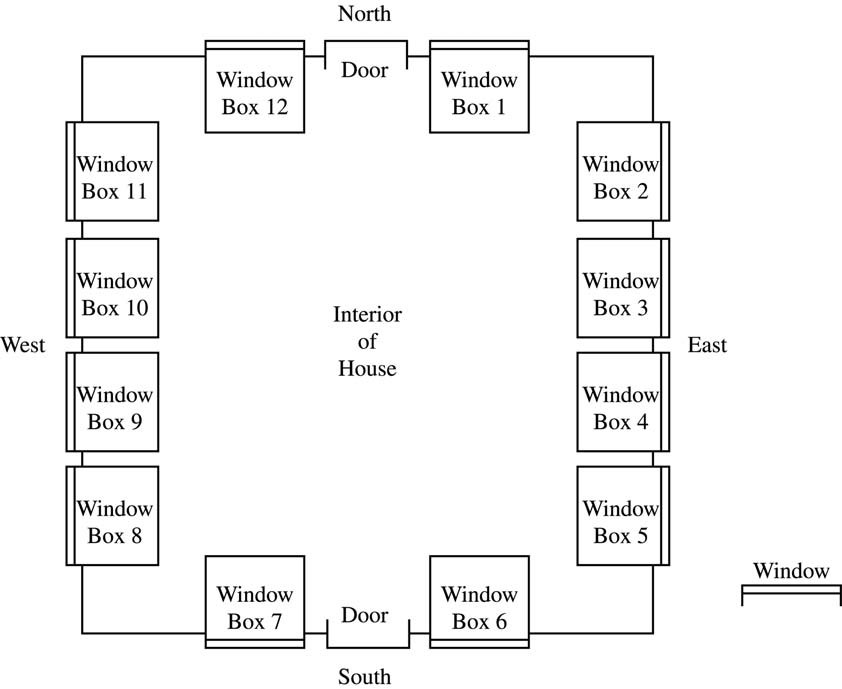
\includegraphics[scale=0.5]{2007FRB3.JPG}
    \end{center}
    In the interior of the house, each window is surrounded by a window box to capture and measure the amount of heat coming in through that window and to isolate the heat gain for each window.
       \begin{enumerate}[label =(\alph*)]
          \item A randomized block experiment will be used to compare the heat gain for the two types (A and B) of windows. How would you group the window boxes into blocks? (Clearly indicate your blocks using the window box numbers.) Justify your choice of blocks.
          \item For the design in part (a), describe how you would assign window types (A and B) to the numbered window boxes.
       \end{enumerate}
\end{enumerate}

\end{document}